\section{创新点描述（与现有量子算法或经典算法的差异与优势）}
若从已有路线出发，本文的创新点应当被理解为“相对创新”而非绝对首创。与经典 LETKF/局地加权路线相比，本文额外引入了可解释的量子相似度结构\cite{hunt2007letkf}；与量子核或量子特征映射路线相比，本文没有停留在相似度矩阵展示，而是把该相似度嵌入局地同化权重\cite{yin2025photonicqkernel,saez2025qkernel,altmann2025qgk}；与量子数据同化或算子代数路线相比，本文没有试图让量子模块整体替代状态估计，而是只让其进入 LETKF 的局地结构层\cite{kotsuki2024qda,giannakis2022operator}。基于这种定位，本文的主要创新点可概括为以下三方面：
\begin{itemize}
\item \textbf{作用位点创新}：相对于仅把量子模块用于超参数搜索的做法，本文把量子信息嵌入到 LETKF 的局地权重与弱方向修正中，使量子模块进入同化公式内部而不是停留在外层；
\item \textbf{表示层创新}：相对于只报告量子核矩阵或相似度矩阵的做法，本文利用局地窗口量子特征映射构造状态--观测相似度，并将其明确解释为局地几何结构编码器；
\item \textbf{融合机制创新}：相对于直接结构化加权或强替代更新的做法，本文采用“距离先验 + 量子相似度”的弱融合方式，并通过小幅 $J$ 修正限制量子信号强度，使量子增强与经典稳定性兼容。
\end{itemize}

如果只把上述三点列成条目，仍然不足以体现本文方法的真正创新性。本文的价值不在于单独提出某一个新公式，而在于把“量子信息如何进入同化器”这一问题拆成了可分析的几个层次，并在每个层次上给出对应的结构解释。换句话说，创新不仅体现在结果更优，也体现在方法的可解释性更完整。

\begin{figure}[htbp]
\centering
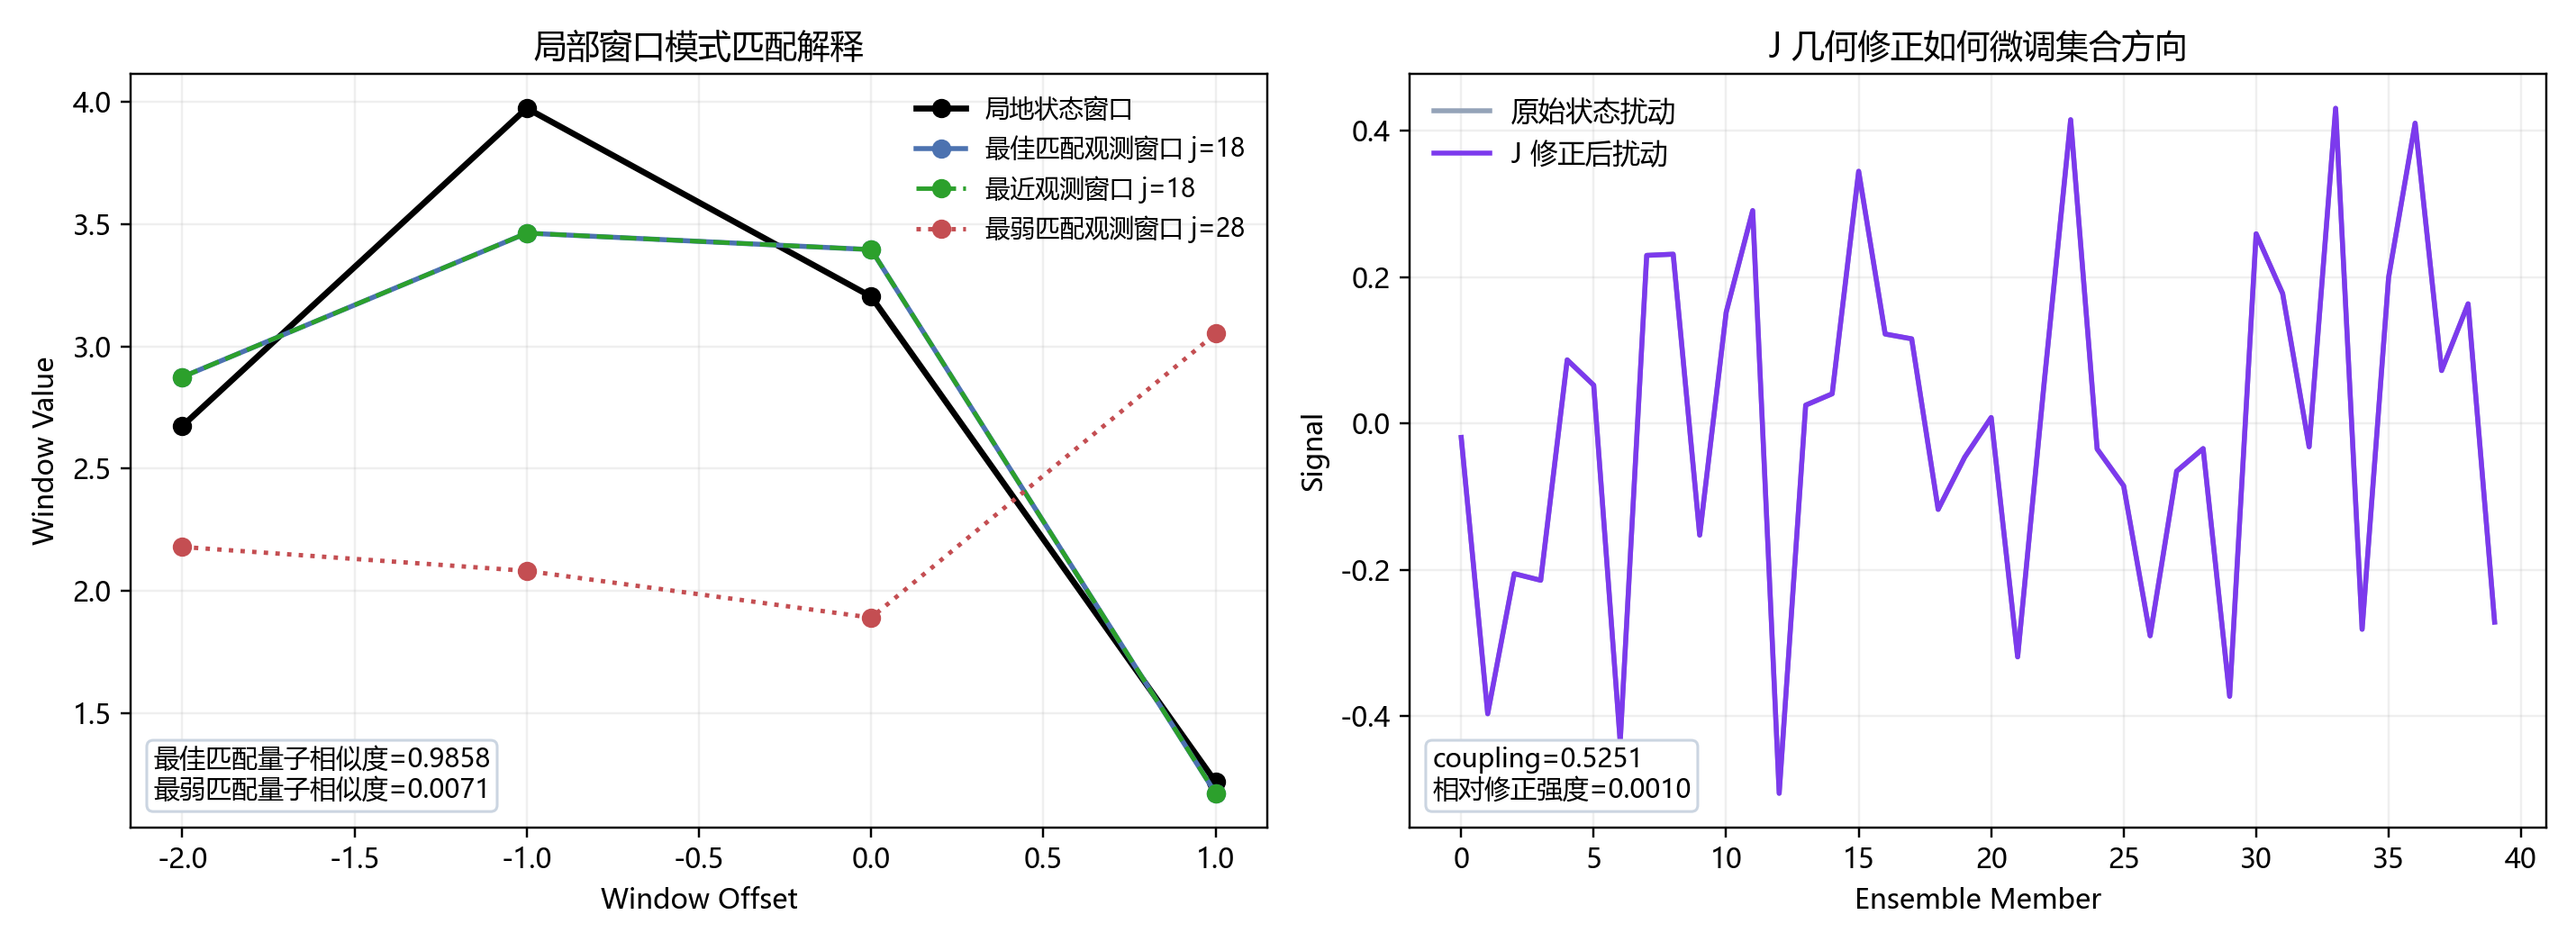
\includegraphics[width=0.92\linewidth]{figures/exp37_local_window_explanation.png}
\caption{代表性局地窗口下的状态模式、观测模式与弱 $J$ 修正示意。}
\label{fig:local}
\end{figure}

图 \ref{fig:local} 是本文创新点最直接的可视化证据。它说明量子模块并不是抽象地输出一个权重系数，而是在局地窗口内刻画状态模式与观测模式的匹配关系，并据此对集合方向做小幅修正。因此，本文最重要的创新不在于“量子线路更复杂”，而在于给出了一个可追踪的信号流：局地窗口 $\rightarrow$ 相似度 $\rightarrow$ 局地模式 $\rightarrow$ 弱修正。

进一步看，图中的局地模式匹配关系说明了一个重要事实：量子模块的价值不在于生成一个全局最优参数，而在于识别哪些局地观测更值得被当前状态窗口强调。也正因为这种匹配关系是局地的、几何的，所以弱 $J$ 修正必须保持小幅，否则就会把原本有价值的局地提示放大成不稳定的全局扰动。

这也是本文“可解释性”最核心的一层。传统上，量子模块很容易被理解为一个难以分析的黑箱相似度生成器，但图 \ref{fig:local} 说明它其实有非常明确的角色分工：一部分作用于识别局地窗口之间的结构相近性，另一部分作用于判断集合扰动方向是否应被轻微修正。也就是说，量子模块输出的不是不可追踪的神秘特征，而是可以通过局地窗口、模式匹配和方向变化三步解释清楚的结构信号。

\begin{figure}[htbp]
\centering
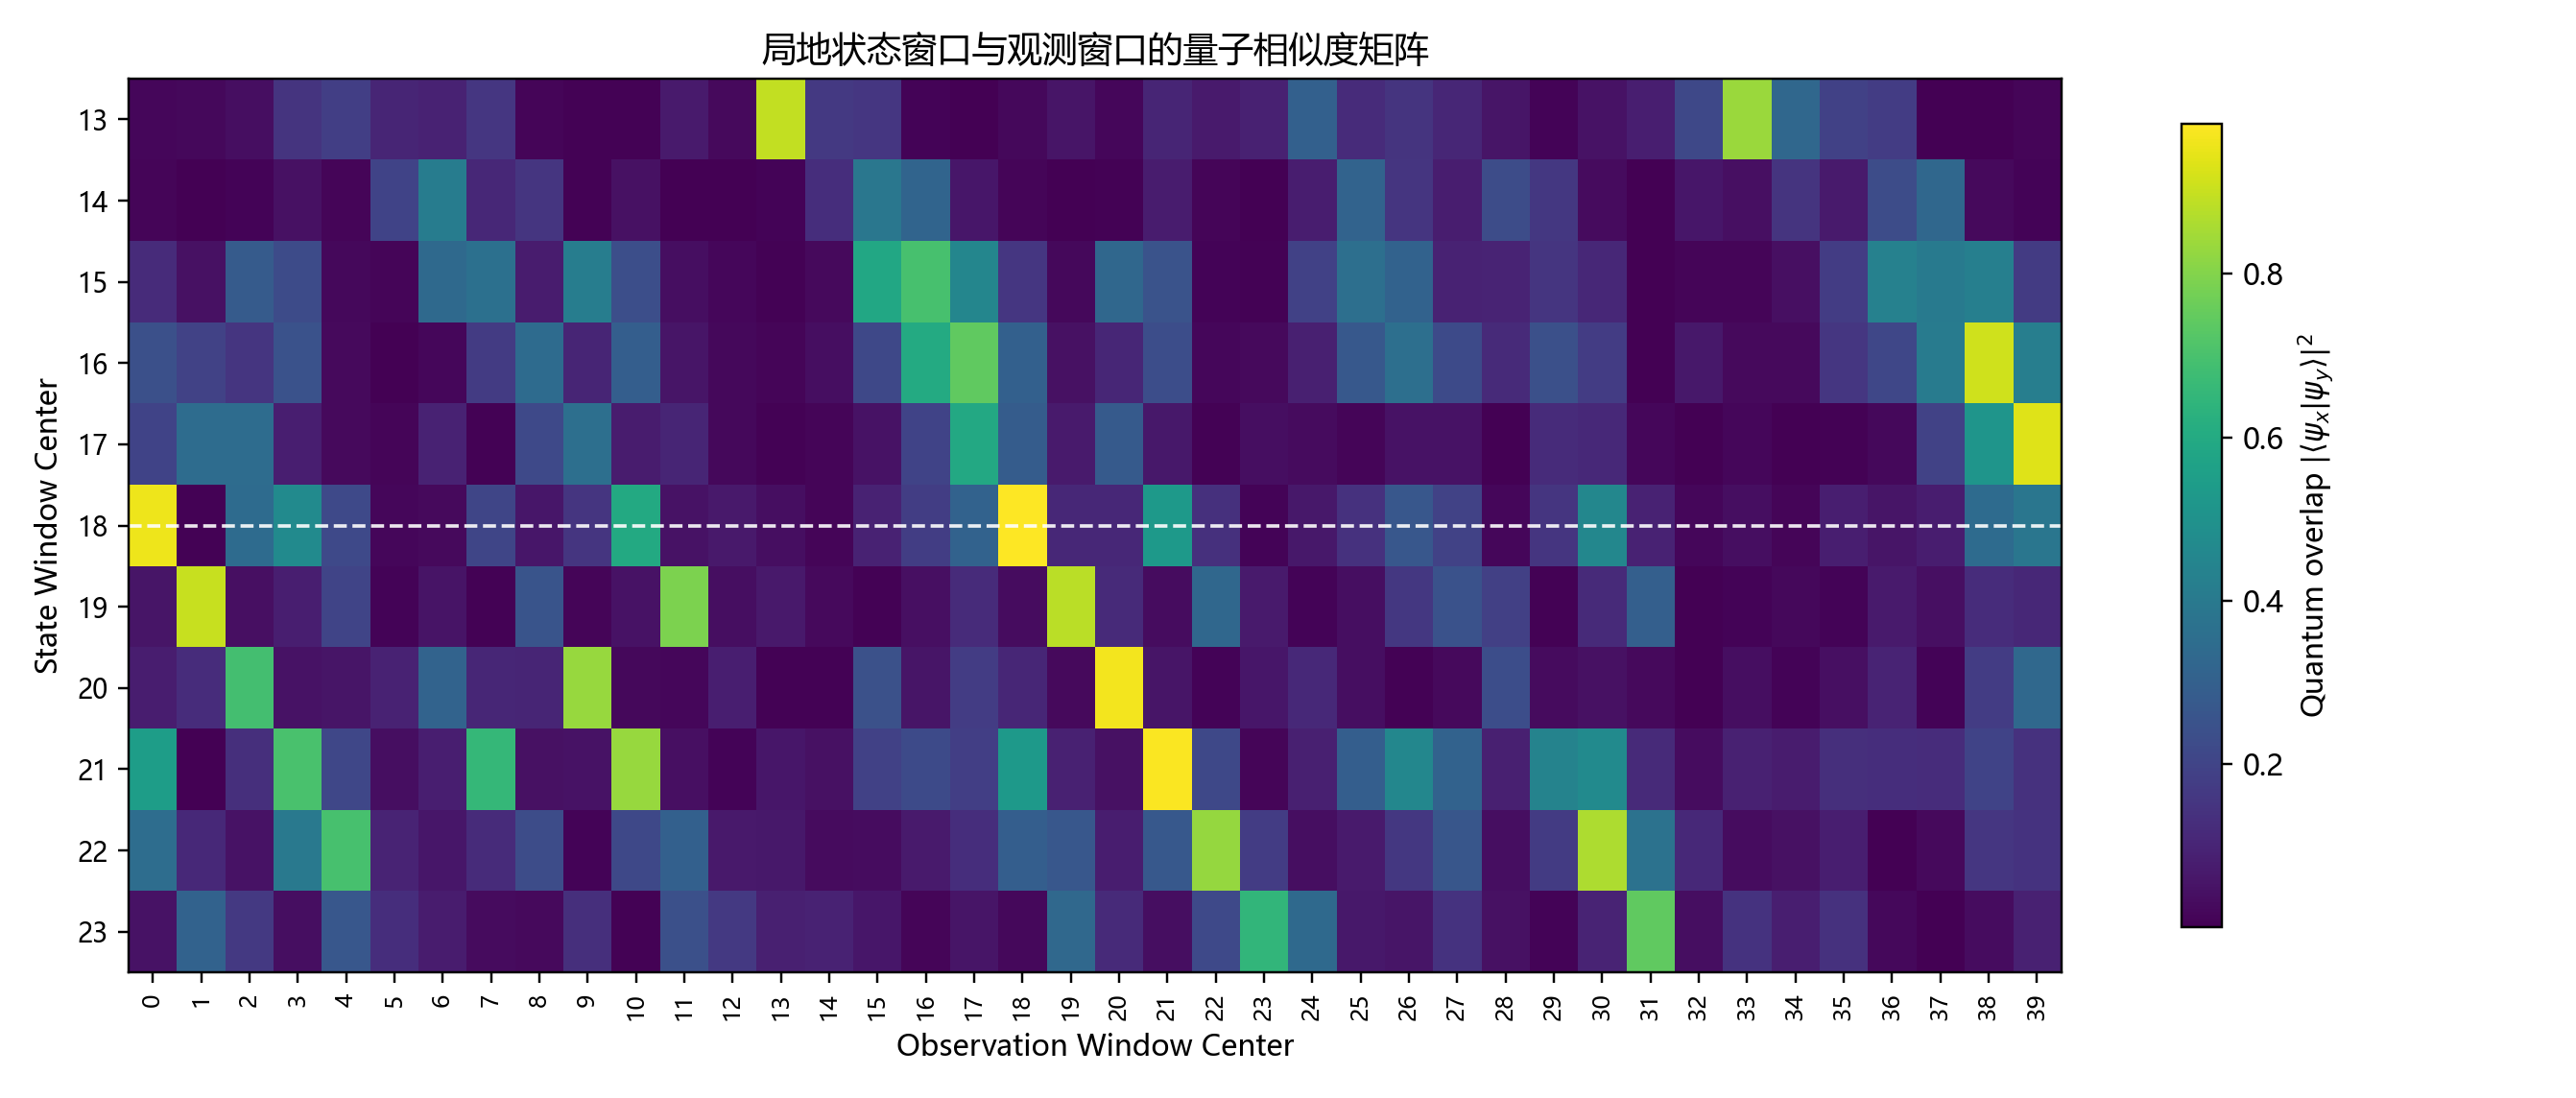
\includegraphics[width=0.92\linewidth]{figures/exp37_quantum_similarity_matrix.png}
\caption{代表性时间步下量子相似度的结构分布。}
\label{fig:qsim-innov}
\end{figure}

图 \ref{fig:qsim-innov} 进一步加强了这种解释性。该图显示，不同局地窗口之间的相似度并不是均匀或随机的，而是呈现出明显的块状和层次差异。这说明量子模块确实学习到了一种局地结构表达，而不是简单复述经典距离先验。若没有这层结构差异，后续的弱融合权重就不可能在保持稳定的同时提供额外信息。就本文当前实验而言，这种“结构表达创新”是有证据支持的；但是否能推广到更复杂系统和更大窗口，仍需后续工作检验。这里与现有量子核文献的关键差别在于，已有工作更多关注分类、回归或核分离能力\cite{yin2025photonicqkernel,saez2025qkernel}，而本文把量子相似度放进了局地同化加权这一更具体的动力系统任务中。

因此，本文的创新点可以进一步概括为三条解释链。第一条是“局地窗口解释链”，说明量子模块为何适合处理局地模式匹配；第二条是“相似度解释链”，说明量子特征映射为何能产生非平凡结构信息；第三条是“弱修正解释链”，说明这些结构信息为何必须以弱融合和弱 $J$ 修正的形式进入经典同化器。三条解释链共同决定了本文不是简单堆叠量子术语，而是在方法、结构和行为三个层次上都可解释。不过从学术表述上讲，本文更适合声称“在当前受控实验中建立了一套可解释的量子弱融合机制”，而不是直接宣称已经给出普适方法论。
